%Este trabalho está licenciado sob a Licença Creative Commons Atribuição-CompartilhaIgual 3.0 Não Adaptada. Para ver uma cópia desta licença, visite http://creativecommons.org/licenses/by-sa/3.0/ ou envie uma carta para Creative Commons, PO Box 1866, Mountain View, CA 94042, USA.

%\documentclass[main.tex]{subfiles}
%\begin{document}

\chapter{Ajuste de curvas}\index{aproximação!de funções}\index{ajuste!por mínimos quadrados}

Neste capítulo, discutimos sobre problemas de \emph{ajuste de curvas}\index{ajuste de curvas} pelo \emph{método dos mínimos quadrados}\index{método dos mínimos quadrados}. Mais precisamente, dado um conjunto de $N$ pontos $\left\{(x_j, y_j)\in \mathbb{R}^2\right\}_{j=1}^N$ e uma família de funções $\mathcal{F} = \{f:\mathbb{R}\to\mathbb{R}; y = f(x)\}$, o problema de ajuste de curvas consiste em encontrar uma função da família $\mathcal{F}$ que melhor se ajusta aos pontos dados, não necessariamente que os interpola. 

\begin{figure}[h!]
  \centering
  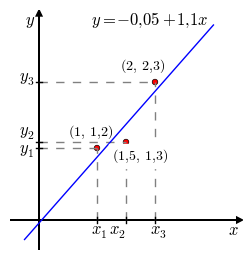
\includegraphics[scale=0.9]{./cap_ajuste/pics/ex_intro_ajuste/ex_intro_ajuste}
  \caption{Exemplo de um problema de ajuste de uma reta entre três pontos, veja o exemplo~\ref{ex:intro_ajuste}.}
  \label{fig:ex_intro}
\end{figure}

Aqui, o termo ``melhor se ajusta'' é entendido no sentido de mínimos quadrados, isto é, buscamos encontrar uma função $f\in\mathcal{F}$ tal que $f(x)$ resolve o seguinte problema de minimização
\begin{equation*}
  \min_{f\in\mathcal{F}} \sum_{j=1}^N \left(f(x_j) - y_j\right)^2,
\end{equation*}
ou seja, $f(x)$ é a função da família $\mathcal{F}$ cujo erro quadrático entre $y_j$ e $f(x_j)$, $j = 1, 2, \dotsc, N$, é mínimo. A expressão
\begin{equation*}
  \begin{split}
  R &:= \sum_{j=1}^N \left(f(x_j)-y_j\right)^2 \\
  &= \left(f(x_1)-y_1\right)^2 +  \left(f(x_2)-y_2\right)^2 + \cdots + \left(f(x_N)- y_N\right)^2    
  \end{split}
\end{equation*}
é chamada de \emph{resíduo}\index{resíduo} e consiste na soma dos quadrados das diferenças entre a ordenadas $y_j$ e o valor da função procurada $f(x_j)$.

\begin{ex}\label{ex:intro_ajuste}
  Dado o conjunto de pontos $\{(1, 1,2)$, $(1,5, 1,3)$, $(2, 2,3)\}$ e a família de retas $f(x) = a + bx$, podemos mostrar que $f(x) = -0,05 + 1,1x$ é a reta que melhor aproxima os pontos dados no sentido de mínimos quadrados.  Os pontos e a reta ajustada e são esboçados na figura~\ref{fig:ex_intro}.
\end{ex}

Na sequência, discutimos o procedimento de ajuste de uma reta, então, mostramos a generalização da técnica para problemas lineares de ajuste e, por fim, discutimos alguns problemas de ajuste não lineares.

%%%%%%%%%%%%%%%%%%%%
% python
%%%%%%%%%%%%%%%%%%%%
\ifispython
  Ao longo deste capítulo, estaremos assumindo que as seguintes bibliotecas e módulos \verb+Python+ estão carregadas:
\begin{verbatim}
>>> from __future__ import division
>>> import numpy as np
>>> from numpy import linalg
>>> import matplotlib.pyplot as plt
\end{verbatim}
\fi
%%%%%%%%%%%%%%%%%%%%


\section{Ajuste de uma reta}\index{ajuste!de uma reta}

Nesta seção, discutiremos o procedimento de ajuste de uma reta a um conjunto de pontos dados. Em outras palavras, discutiremos o método de solução para o problema de encontrar o polinômio do primeiro grau que melhor se aproxima a um dado conjunto de pontos pelo método dos mínimos quadrados. 

Seja, então, $\{(x_1,y_1), (x_2,y_2),\ldots, (x_N,y_N)\}$ um conjunto de $N$ pontos dados. Buscamos encontrar a função $f(x) = a_1 + a_2x$ tal que o resíduo
\begin{equation*}
  R = \sum_{j=1}^N (f(x_j)-y_j)^2
\end{equation*}
seja mínimo.

Para tal, primeiro observamos que $f(x_j)=a_1+a_2 x_j$ e, portanto, o resíduo pode ser escrito explicitamente como uma função de $a_1$ e $a_2$ conforme a seguinte expressão:
\begin{equation*}
  R(a_1,a_2) = \sum_{j=1}^N (a_1 + a_2x_j - y_j)^2.
\end{equation*}

%O objetivo é encontrar $a_1, a_2$ e geralmente temos muito mais equações do que incógnitas, isto é,
%\begin{eqnarray*}
% a_1+a_2 x_1 &=&y_1 \\
% a_1+a_2 x_2 &=&y_2 \\
% a_1+a_2 x_3 &=&y_3 \\
%  \vdots     &=& \vdots \\
% a_N+a_2 x_N &=&y_N   
%\end{eqnarray*}
%ou simplesmente $V\vec a= \vec y$.

Observamos que $R(a_1,a_2)$ é uma forma quadrática e que seu mínimo ocorre quando suas derivadas parciais primeiras são iguais a zero, isto é,
\begin{eqnarray*}
  \frac{\partial R}{\partial a_1} &=& \frac{\partial }{\partial a_1} \sum_{j=1}^N (a_1 + a_2 x_j-y_j)^2 =0, \\
  \frac{\partial R}{\partial a_2} &=& \frac{\partial }{\partial a_2} \sum_{j=1}^N (a_1 + a_2 x_j-y_j)^2 =0. 
\end{eqnarray*}
Ou seja,
\begin{eqnarray*}
   2 \sum_{j=1}^N (a_1 + a_2 x_j-y_j)\cdot 1 &=&0, \\
   2 \sum_{j=1}^N (a_1 + a_2 x_j-y_j)\cdot x_j &=&0, 
\end{eqnarray*}
e isolando as incógnitas temos
\begin{eqnarray*}
   a_1\sum_{j=1}^N 1 + a_2 \sum_{j=1}^Nx_j &=&\sum_{j=1}^N y_j,\\
   a_1\sum_{j=1}^N x_j + a_2 \sum_{j=1}^Nx_j^2 &=&\sum_{j=1}^N y_jx_j.
\end{eqnarray*}
Observando que $\sum_{j=1}^N 1=N$, o sistema linear acima pode ser escrito na forma matricial $Ma = w$, isto é,
\begin{equation}\label{eq:smq_reta}
  \underbrace{\begin{bmatrix}
     N &  \sum_{j=1}^N x_j \\
     \sum_{j=1}^N x_j &  \sum_{j=1}^N x_j^2 
  \end{bmatrix}}_{M}
  \underbrace{\begin{bmatrix}
     a_1 \\
     a_2 
  \end{bmatrix}}_{a} =
  \underbrace{\begin{bmatrix}
     \sum_{j=1}^N y_j \\
     \sum_{j=1}^N x_j y_j 
  \end{bmatrix}}_{w}.
\end{equation}

Este sistema linear de duas equações e duas incógnitas admite uma única solução quando o determinante da matriz dos coeficientes for não nulo, isto é,  
\begin{eqnarray*}
N \sum_{j=1}^N x_j^2 - \left(\sum_{j=1}^N x_j\right)^2 \neq 0 
\end{eqnarray*}

Pode-se mostrar usando a \emph{desigualdade de Cauchy–Schwarz} que isto acontece quando existem pelo menos duas abscissas diferentes envolvidas no ajuste.  Usando a fórmula da inversa de uma matriz dois-por-dois, chegamos às seguintes fórmulas para os coeficientes $a_1$ e $a_2$:
  \begin{equation}\label{eq:formula_final_ajuste_reta}
    \begin{split}
    a_1 &= \frac{\sum_{j=1}^N x_j^2  \cdot \sum_{j=1}^N y_j - \sum_{j=1}^N x_j \cdot \sum_{j=1}^N x_jy_j}{N \sum_{j=1}^N x_j^2 - \left(\sum_{j=1}^N x_j\right)^2}\\
    a_2 &= \frac{N \sum_{j=1}^N x_jy_j - \sum_{j=1}^N x_j  \cdot \sum_{j=1}^N y_j }{N \sum_{j=1}^N x_j^2 - \left(\sum_{j=1}^N x_j\right)^2}      
    \end{split}
\end{equation}

Por fim, observamos que o sistema $Ma = w$ descrito na equação~\eqref{eq:smq_reta} pode ser reescrito na forma $V^TVa = V^Ty$, onde $V := [1~x]$ é a matriz dos coeficientes do seguinte sistema linear sobre determinado:
\begin{equation}\label{eq:smq_reta2}
  \begin{split}
  a_1 + a_2x_1 &= y_1\\
  a_1 + a_2x_2 &= y_2\\
  &\vdots\\
  a_1 + a_2x_N &= y_N
  \end{split}
\end{equation}
Se os pontos dados não são colineares, este sistema não têm solução. Mas, sempre que pelo menos duas abscissas foram diferentes, $M = V^TV$ é uma matriz invertível e (veja o exercício~\ref{exer:smq_reta}), então
\begin{equation}\label{eq:sol_smq_reta}
  a = \left(V^TV\right)^{-1}V^Ty,
\end{equation}
nos fornece a chamada solução por mínimos quadrados do sistema \eqref{eq:smq_reta2}. Note que esta é uma forma de se obter os coeficientes $a = (a_1, a_2)$ equivalente àquela dada em \eqref{eq:formula_final_ajuste_reta}.


\begin{ex}\label{ex:calculo_intro_ajuste}
  Retornemos ao exemplo \ref{ex:intro_ajuste}. Isto é, dado o conjunto de pontos $\{(1, 1,2)$, $(1,5, 1,3)$, $(2, 2,3)\}$, encontrar a função do tipo $f(x) = a_1 + a_2x$ que melhor se ajusta os pontos dados no sentido de mínimos quadrados.
\end{ex}
\begin{sol} Usando as fórmulas em \eqref{eq:formula_final_ajuste_reta}, obtemos
  \begin{eqnarray*}
    a_1&=&\frac{7,25 \cdot 4,8 - 4,5 \cdot 7,75  }{3\cdot 7,25 - 20,25 } = -0,05, \\
    a_2&=&\frac{3\cdot 7,75 - 4,5\cdot 4,8}{3\cdot 7,25 - 20,25}=1,1.
  \end{eqnarray*}
Ou seja, verificamos que, de fato, a função $f(x) = -0,05 + 1,1x$ corresponde à reta que melhor ajusta os pontos dados no sentido de mínimos quadrados. Os pontos e a reta ajustada estão esboçados na figura~\ref{fig:ex_intro}.

Deixamos ao leitor a verificação de que os coeficientes $a_1$ e $a_2$ também podem ser obtidos pela expressão~\eqref{eq:sol_smq_reta}.

%%%%%%%%%%%%%%%%%%%%
% scilab
%%%%%%%%%%%%%%%%%%%%
\ifisscilab
Os coeficientes $a_1$ e $a_2$ podem ser rapidamente calculados no \verb+Scilab+ usando a expressão~\eqref{eq:sol_smq_reta}. Para tando, digitamos:
\begin{verbatim}
-->xj = [1, 1.5, 2]';  
-->yj = [1.2, 1.3, 2.3]'; 
-->V = [ones(3,1) xj]; 
-->a = inv(V'*V)*V'*yj 
 a  =
  - 0.05  
    1.1   
\end{verbatim}
Então, o gráfico da função ajustada e dos pontos pode ser obtido com os comandos:
\begin{verbatim}
-->deff('y = f(x)','y = a(1) + a(2)*x')
-->xx = linspace(0.5,2.5); 
-->plot(xj,yj,'ro',xx,f(xx),'b-')
\end{verbatim}
\fi
%%%%%%%%%%%%%%%%%%%%
%%%%%%%%%%%%%%%%%%%%
% octave
%%%%%%%%%%%%%%%%%%%%
\ifisoctave
Os coeficientes $a_1$ e $a_2$ podem ser rapidamente calculados no \verb+GNU Octave+ usando a expressão~\eqref{eq:sol_smq_reta}. Para tando, digitamos:
\begin{verbatim}
xj = [1, 1.5, 2]';
yj = [1.2, 1.3, 2.3]';
V = [ones(3,1) xj];
a = inv(V'*V)*V'*yj
\end{verbatim}
o que nos fornece no {\it prompt}:
\begin{verbatim}
 a  =
  - 0.05  
    1.1     
\end{verbatim}
Então, o gráfico da função ajustada e dos pontos pode ser obtido com os comandos:
\begin{verbatim}
f = inline("a(1) + a(2)*x")
xx = linspace(0.5,2.5); 
plot(xj,yj,'ro',xx,f(xx),'b-');grid on
\end{verbatim}
\fi
%%%%%%%%%%%%%%%%%%%%
%%%%%%%%%%%%%%%%%%%%
% python
%%%%%%%%%%%%%%%%%%%%
\ifispython
Em \verb+Python+, podemos computar os coeficientes $a_1$ e $a_2$ da seguinte forma:
\begin{verbatim}
>>> xi = np.array([1, 1.5, 2])
>>> yi = np.array([1.2,1.3,2.3])
>>> V = np.array([xi**1,xi**0]).transpose();V
array([[ 1. ,  1. ],
       [ 1.5,  1. ],
       [ 2. ,  1. ]])
>>> a = ((np.linalg.inv((V.transpose()).dot(V))).dot(V.transpose())).dot(yi);a
array([ 1.1 , -0.05])
\end{verbatim}
Então, o gráfico da função ajustada e dos pontos pode ser obtido com os comandos:
\begin{verbatim}
>>> xx = np.linspace(0.5,2.5)
>>> plt.plot(xi,yi,'ro',xx,np.polyval(a,xx),'b-')
>>> plt.grid();plt.show()
\end{verbatim}
\fi
%%%%%%%%%%%%%%%%%%%%

\end{sol}

O procedimento apresentado de ajuste de uma reta por mínimos quadrados pode ser generalizado para qualquer família de funções que seja um espaço vetorial de dimensão finita. Problemas de ajuste com tais famílias de funções é o que chamamos de problemas de ajuste linear, os quais exploramos em detalhe na próxima seção.

\subsection*{Exercício resolvido}

\begin{exeresol}\label{exer:smq_reta}
  \begin{enumerate}[a)]
  \item Mostre que o sistema linear $Ma = w$ descrito na equação~\ref{eq:smq_reta} pode ser reescrito na forma $V^TVa = V^Ty$, onde $V = [1~x]$.
  \item Mostre que $V$, como definido no item a), tem posto igual a 2 quando pelo menos duas abscissas do conjunto de pontos $\{(x_j, y_j)\}_{j=1}^N$ são diferentes. E, portanto, $M = V^TV$ é uma matriz invertível.
  \end{enumerate}
\end{exeresol}
\begin{resol}
    \begin{enumerate}[a)]
    \item Basta observar que
      \begin{equation*}
        V^TV = \begin{bmatrix}
          1 & 1 \cdots & 1\\
          x_1 & x_2 & \cdots & x_N
        \end{bmatrix}
        \begin{bmatrix}
          1 & x_1\\
          1 & x_2\\
          \vdots & \vdots\\
          1 & x_N
        \end{bmatrix} =
        \begin{bmatrix}
          N &  \sum_{j=1}^N x_j \\
          \sum_{j=1}^N x_j &  \sum_{j=1}^N x_j^2 
        \end{bmatrix} = M
      \end{equation*}
      e
      \begin{equation*}
        V^Ty = \begin{bmatrix}
          1 & 1 \cdots & 1\\
          x_1 & x_2 & \cdots & x_N
        \end{bmatrix}
        \begin{bmatrix}
          y_1\\
          y_2\\
          \vdots\\
          y_N
        \end{bmatrix} = 
        \begin{bmatrix}
          \sum_{j=1}^N y_j \\
          \sum_{j=1}^N x_j y_j 
        \end{bmatrix} = w.
      \end{equation*}
    \item Sejam $x_i\neq x_j$ duas abscissas diferentes. Então, a $i$-ésima e $j$-ésima linhas na matriz $V$ são linearmente independentes e, portanto, o posto de $V$ é igual a 2. Por fim, $V^TV$ é não singular, pois, se $u$ é tal que $V^TVu = 0$, então
      \begin{equation*}
        0 = u^TV^TVu = (Vu)^T(Vu) = (Vu)\cdot (Vu) \Rightarrow Vu = 0.
      \end{equation*}
Agora, $Vu = 0$ é uma combinação linear das linhas de $V$ igual a zero, logo $u = 0$, pois as linhas de $V$ são linearmente independentes como mostrado antes. Concluímos que se $V^TVu = 0$, então $u = 0$, isto é, $V^TV$ é não singular.
    \end{enumerate}
\end{resol}


\subsection*{Exercícios}

\begin{exer}
  Sejam dados o conjunto de pontos $\{(0,23, -0,54)$, $(-0,30, -0,54)$, $(0,04, -0,57)\}$. Encontre a função $f(x) = a_1 + a_2x$ que melhor se ajusta no sentido de mínimos quadrados aos pontos dados. Faça, então, um gráfico com os pontos e o esboço da função ajustada.
\end{exer}
\begin{resp}
    $f(x) = -0,55 -0,01x$.
\end{resp}

\begin{exer}
  Seja dado o conjunto de pontos $\{(-0,35, 0,2)$, $(0,15, -0,5)$, $(0,23, 0,54)$, $(0,35, 0,7)\}$. Encontre a função $f(x) = a_1 + a_2x$ que melhor se ajusta no sentido de mínimos quadrados aos pontos dados. Faça, então, um gráfico com os pontos e o esboço da função ajustada.
\end{exer}
\begin{resp}
    $f(x) = 0,19 - 0,47x$.
\end{resp}

\begin{exer}
  Seja dado o conjunto de pontos $\{(-1,94, 1,02)$, $(-1,44, 0,59)$, $(0,93, -0,28)$, $(1,39, -1,04)\}$. Encontre a função $f(x) = a_1 + a_2x$ que melhor se ajusta no sentido de mínimos quadrados aos pontos dados. Então, responda cada item:
  \begin{enumerate}[a)]
  \item Encontre o valor de $f(1)$.
  \item Encontre o valor de $f(0,93)$.
  \item Encontre o valor de $|f(0,93) - (- 0,28)|$.
  \item Encontre o valor do resíduo $R = \sum_{j=1}^N (f(x_j)-y_j)^2$.
  \end{enumerate}
Forneça os valores calculados com $7$ dígitos significativo por arredondamento.
\end{exer}
\begin{resp}
    a)~$-0,6025387$; b)~$-0,5651848$; c)~$0,2851848$; d)~$0,1488041$.
\end{resp}

\section{Ajuste linear geral}\index{ajuste!linear}

O problem geral de ajuste linear consiste em dada uma família $\mathcal{F}$ gerada pelo conjunto de $m$ funções $\{f_1(x), f_2(x), \dotsc, f_m(x)\}$ e um conjunto de $n$ pontos $\{(x_1, y_1)$, $(x_2, y_2)$, $\ldots$, $(x_n, y_n)\}$, calcular os coeficientes $a_1$, $a_2$, $\ldots$, $a_m$ tais que a função dada por
\begin{equation*}
  f(x) = \sum_{j=1}^m a_jf_j(x) = a_1f_1(x)+a_2f_2(x)+\ldots+a_mf_m(x)
\end{equation*}
minimiza o resíduo
\begin{equation*}
  R= \sum_{i=1}^n \left[f(x_i)-y_i\right]^2.
\end{equation*}
Aqui, a minimização é feita por todas as possíveis escolhas dos coeficientes $a_1$, $a_2$, $\ldots$, $a_m$.

Com o objetivo de tornar a desenvolvimento mais claro, vamos escrever $R$ como a soma dos resíduos parciais:
\begin{equation*}
  R= \sum_{i=1}^n R_i,\quad \text{onde} \quad R_i := \left[f(x_i)-y_i\right]^2.
\end{equation*}
Do fato que $f(x_i)=\sum_{j=1}^m a_jf_j(x_i)$, temos que cada resíduo pode ser escrito como
\begin{equation*}
  R_i=  \left[\sum_{j=1}^m a_jf_j(x_i)-y_i\right]^2.
\end{equation*}

A fim de encontrar o ponto de mínimo, resolvemos o sistema oriundo de igualar a zero cada uma das derivadas parciais de $R$ em relação aos $m$ coeficientes $a_j$, isto é, devemos resolver:
\begin{eqnarray*}
\frac{\partial R}{\partial a_1} &=& 2 \sum_{i=1}^n \frac{\partial R_i}{\partial a_1} = 2\sum_{i=1}^n \left[\sum_{j=1}^m a_jf_j(x_i)-y_i\right] f_1(x_i)=0,\\
\frac{\partial R}{\partial a_2} &=& 2 \sum_{i=1}^n \frac{\partial R_i}{\partial a_2}=2\sum_{i=1}^n \left[\sum_{j=1}^m a_jf_j(x_i)-y_i\right] f_2(x_i)=0,\\
&\vdots&\\
\frac{\partial R}{\partial a_m} &=& 2 \sum_{i=1}^n \frac{\partial R_i}{\partial a_m}= 2\sum_{i=1}^n \left[\sum_{j=1}^m a_jf_j(x_i)-y_i\right] f_m(x_i)=0.
\end{eqnarray*}

Dividindo cada equação por 2 e escrevendo na forma matricial, obtemos $Ma=w$, onde a matriz $M$ é dada por:
\begin{eqnarray*}
M = \begin{bmatrix}
\sum\limits_{i=1}^n f_1(x_i)^2 & \sum\limits_{i=1}^n f_2(x_i) f_1(x_i) & \!\cdots\! & \sum\limits_{i=1}^n f_m(x_i) f_1(x_i)\\
\sum\limits_{i=1}^n f_1(x_i) f_2(x_i)&\sum\limits_{i=1}^n f_2(x_i)^2 & \!\cdots\! & \sum\limits_{i=1}^n f_m(x_i)  f_2(x_i)\\
\sum\limits_{i=1}^n f_1(x_i) f_3(x_i)&\sum\limits_{i=1}^n f_2(x_i)f_3(x_i) & \!\cdots\! & \sum\limits_{i=1}^n f_m(x_i)  f_3(x_i)\\
\vdots & \vdots & \ddots & \vdots\\
\sum\limits_{i=1}^n f_1(x_i) f_m(x_i)&\sum\limits_{i=1}^n f_2(x_i)f_m(x_i) & \!\cdots\! & \sum\limits_{i=1}^n f_m(x_i)  ^2
\end{bmatrix}.
\end{eqnarray*}
E os vetores $a$ e $w$, por:
\begin{eqnarray*}
a=\left[
\begin{array}{c}
a_1\\
a_2\\
\vdots\\
a_m
\end{array}
\right]\qquad\text{e}\qquad w=\left[\begin{array}{c}
\sum\limits_{i=1}^n f_1(x_i) y_i\\
\sum\limits_{i=1}^n f_2(x_i) y_i\\
\sum\limits_{i=1}^n f_3(x_i) y_i\\
\vdots\\
\sum\limits_{i=1}^n f_m(x_i) y_i
\end{array}
\right]
\end{eqnarray*}

Agora, observamos que $M=V^TV$ e $w=V^T y$, onde a matriz $V$ é dada por:
\begin{equation*}
  V=\begin{bmatrix}
    f_1(x_1)&f_2(x_1) & \cdots & f_m(x_1)\\
    f_1(x_2)&f_2(x_2) & \cdots & f_m(x_2)\\
    f_1(x_3)&f_2(x_3) & \cdots & f_m(x_3)\\
    \vdots & \vdots & \ddots & \vdots\\
    f_1(x_n)&f_2(x_n) & \cdots & f_m(x_n)
  \end{bmatrix}
\end{equation*}
e é o vetor coluna $y = (y_1, y_2, \dotsc, y_N)$,

Então, o problema de ajuste se reduz a resolver o sistema linear $Ma=w$, ou $V^TVa = V^T y$. Este sistema linear tem solução única se a matriz $M$ for inversível. O teorema a seguir mostra que isto acontece sempre a matriz $V$ possui posto $m$, ou seja, o número de linhas linearmente independentes for igual ao número de colunas.\footnote{Nota-se que o posto não pode ultrapassar o número de colunas.}


\begin{teo}
A matriz $M=V^TV$ é quadrada de ordem $m$ e é inversível sempre que o posto da matriz $V$ é igual a número de colunas $m$.
\end{teo}
\begin{proof}
Para provar que $M$ é inversível, precisamos mostrar que se $v$ é um vetor de ordem $m$ e $Mv=0$, então $v=0$. Suponha, então, que $Mv=0$, isto é, 
$V^TVv=0$. Tomando o produto interno da expressão $V^TVv=0$ com $v$, temos:
$$0=\left<V^TVv,v\right>=\left<Vv,Vv\right>=\|Vv\|^2$$
Portato $Mv=0$ implica obrigatoriamente $Vv=0$. Como o posto de $V$ é igual ao número de colunas, $v$ precisar ser o vetor nulo.
\end{proof}
%\begin{lem}
% A matriz $M=V^TV$ é simétrica.
%\end{lem}
%\begin{proof}
%Isso é facilmente provado pelo seguinte argumento:
%$$M^T=(V^TV)^T=(V)^T(V^T)^T=V^TV=M$$
%\end{proof}

\begin{obs} Este problema é equivalente a resolver pelo métodos dos mínimos quadrados o seguinte sistema linear:
  \begin{equation*}
    \begin{bmatrix}
      f_1(x_1)&f_2(x_1) & \cdots & f_m(x_1)\\
      f_1(x_2)&f_2(x_2) & \cdots & f_m(x_2)\\
      f_1(x_3)&f_2(x_3) & \cdots & f_m(x_3)\\
      \vdots & \vdots & \ddots & \vdots\\
      f_1(x_n)&f_2(x_n) & \cdots & f_m(x_n)
    \end{bmatrix}
    \begin{bmatrix}
      a_1\\
      a_2\\
      \vdots\\
      a_m
    \end{bmatrix}
    =\begin{bmatrix}
      y_1\\
      y_2\\
      y_3\\
      \vdots\\
      y_n
    \end{bmatrix}
  \end{equation*}
\end{obs}

O caso de ajuste de um reta para um conjunto de pontos é um caso particular de ajuste linear.

\begin{figure}
  \centering
  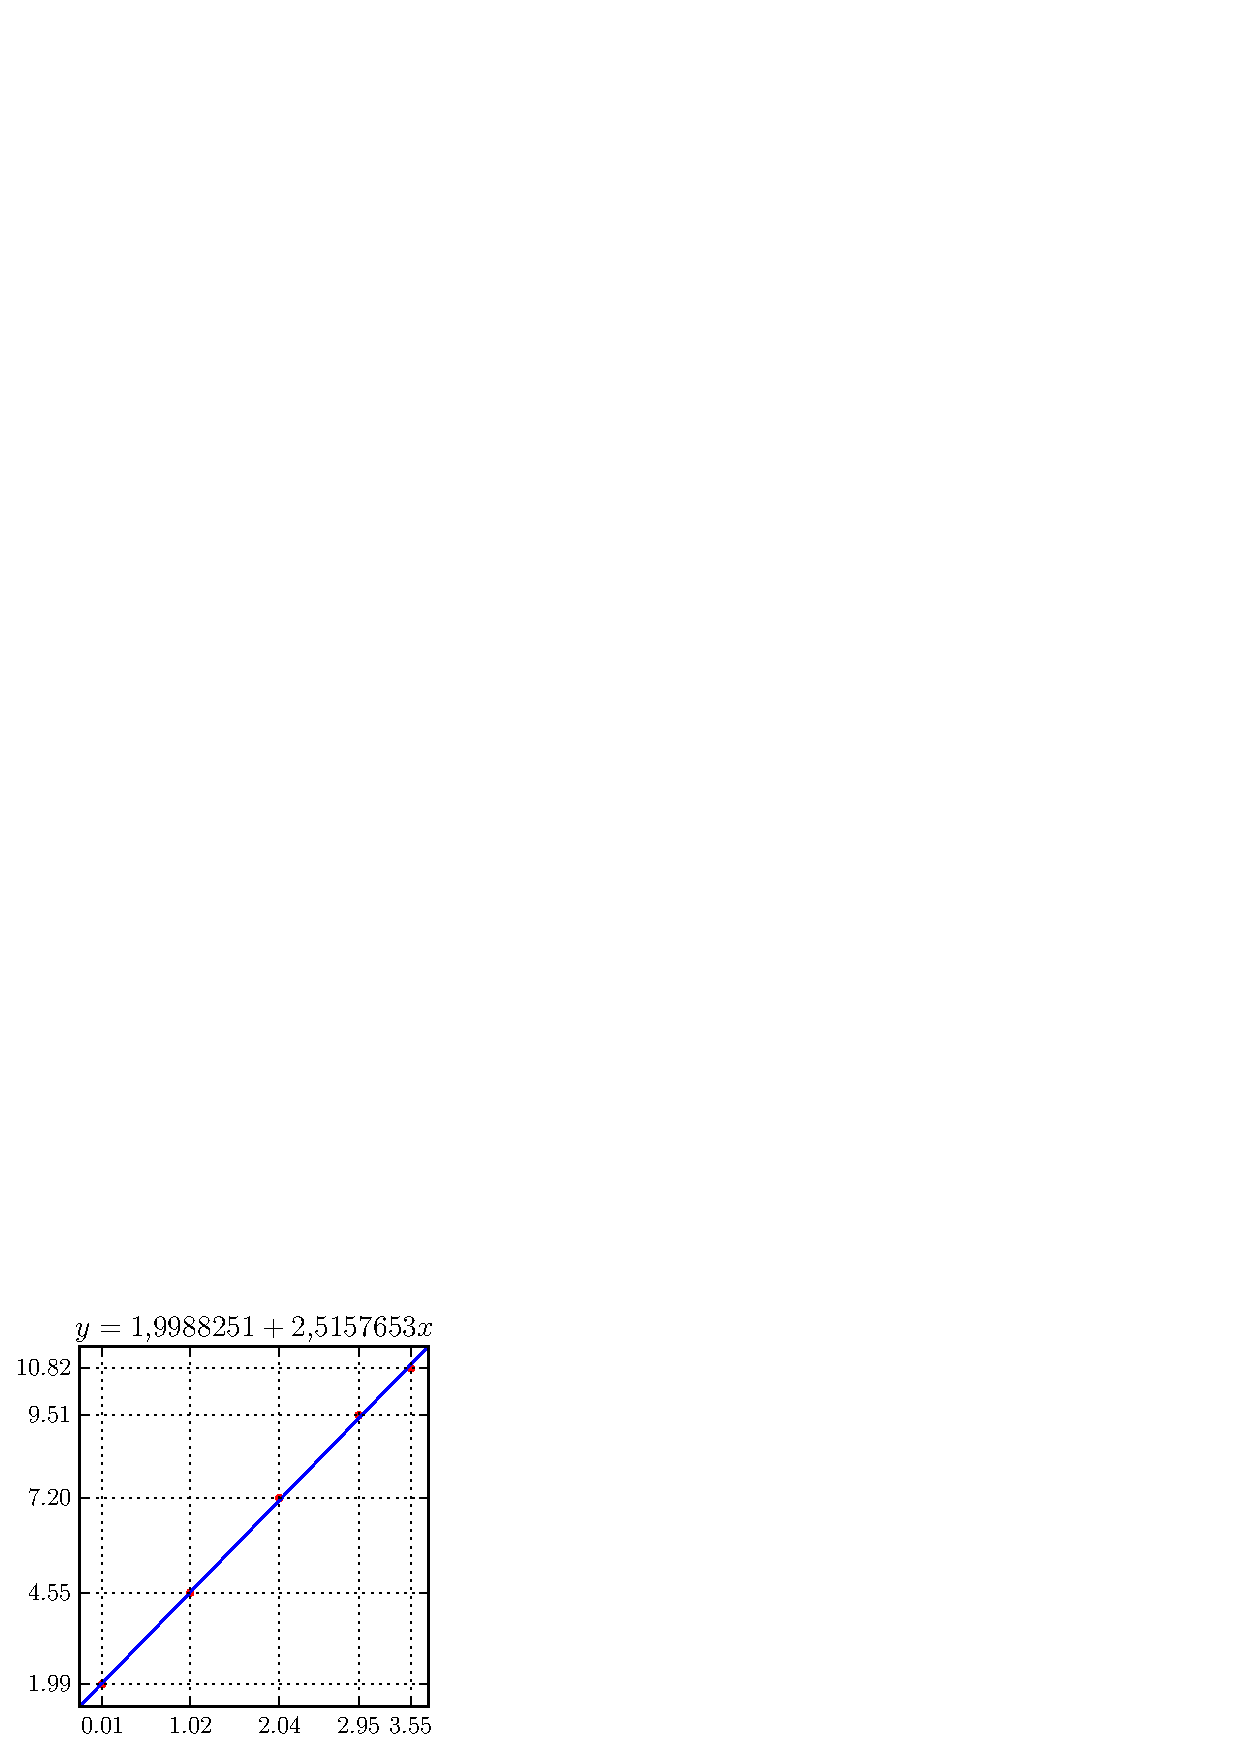
\includegraphics{cap_ajuste/pics/ex_ajuste_reta2/ex_ajuste_reta2}
  \caption{Gráfico da solução do problema apresentado no exemplo~\ref{ex:ajuste_reta2}.}
  \label{fig:ex_ajuste_reta2}
\end{figure}

\begin{ex}\label{ex:ajuste_reta2} Encontre a reta que melhor se ajusta aos pontos dados na seguinte tabela:
  \begin{center}
    \begin{tabular}{l|ccccc}
      $i$ & $1$   & $2$  & $3$ & $4$ & $5$\\\hline
      $x_i$& $0,01$ & $1,02$ & $2,04$ & $2,95$ & $3,55$\\
      $y_i$ & $1,99$ & $4,55$ & $7,20$ & $9,51$ & $10,82$
    \end{tabular}
  \end{center}
\end{ex}
\begin{sol}
O problema consiste em ajustar uma função da forma $f(x) = a_1 + a_2x$ no conjunto de pontos dados. Notamos que $f(x)$ é uma função da família gerada pelo conjunto de funções $\{f_1(x) = 1, f_2(x) = x\}$. Então, aplicando o procedimento acima, temos que o vetor dos coeficientes $a = (a_1, a_2)$ é solução por mínimos quadrados do sistema linear $Va = y$, onde:
\begin{equation*}
  V = \begin{bmatrix}
    f_1(x_1) & f_2(x_1)\\
    f_1(x_2) & f_2(x_2)\\
    f_1(x_3) & f_2(x_3)\\
    f_1(x_4) & f_2(x_4)\\
    f_1(x_5) & f_2(x_5)
  \end{bmatrix}
= \begin{bmatrix}
    1 &0,01\\
    1 &1,02\\
    1 &2,04\\
    1 &2,95\\
    1 &3,55
\end{bmatrix}.
\end{equation*}
Ou seja, é a solução do sistema $V^TVa = V^Ty$ dado por
\begin{equation*}
  \begin{bmatrix}
    5     & 9,57 \\
    9,57  & 26,5071
  \end{bmatrix}
  \begin{bmatrix}
    a_1   \\
    a_2
  \end{bmatrix}=
  \begin{bmatrix}
    34,07  \\
    85,8144
  \end{bmatrix}
\end{equation*}
A solução desse sistema é $a_1 = 1,9988251$ e $a_2 = 2,5157653$. A figura~\ref{fig:ex_ajuste_reta2}, apresenta um gráfico dos pontos e da reta ajustada.

% A tabela abaixo mostra os valores dados e os valores ajustados:
% \begin{center}
% \begin{tabular}{|c|c|c|c|}
% \hline
% $x_i$ & $y_i$& $ax_i+b$& $ax_i+b-y_i$\\
% \hline
% $0,01$ & $1,99$ & $2,0239828$ & $0,0339828$\\
% $1,02$ & $4,55$ & $4,5649057$ & $0,0149057$ \\
% $2,04$ & $7,2$ & $7,1309863$ & $-0,0690137$ \\
% $2,95$ & $9,51$ & $9,4203327$ & $-0,0896673$  \\
% $3,55$ & $10,82$ & $10,929792$ & $0,1097919$ \\
% \hline
% \end{tabular}  
% \end{center}
\end{sol}

\begin{figure}
  \centering
  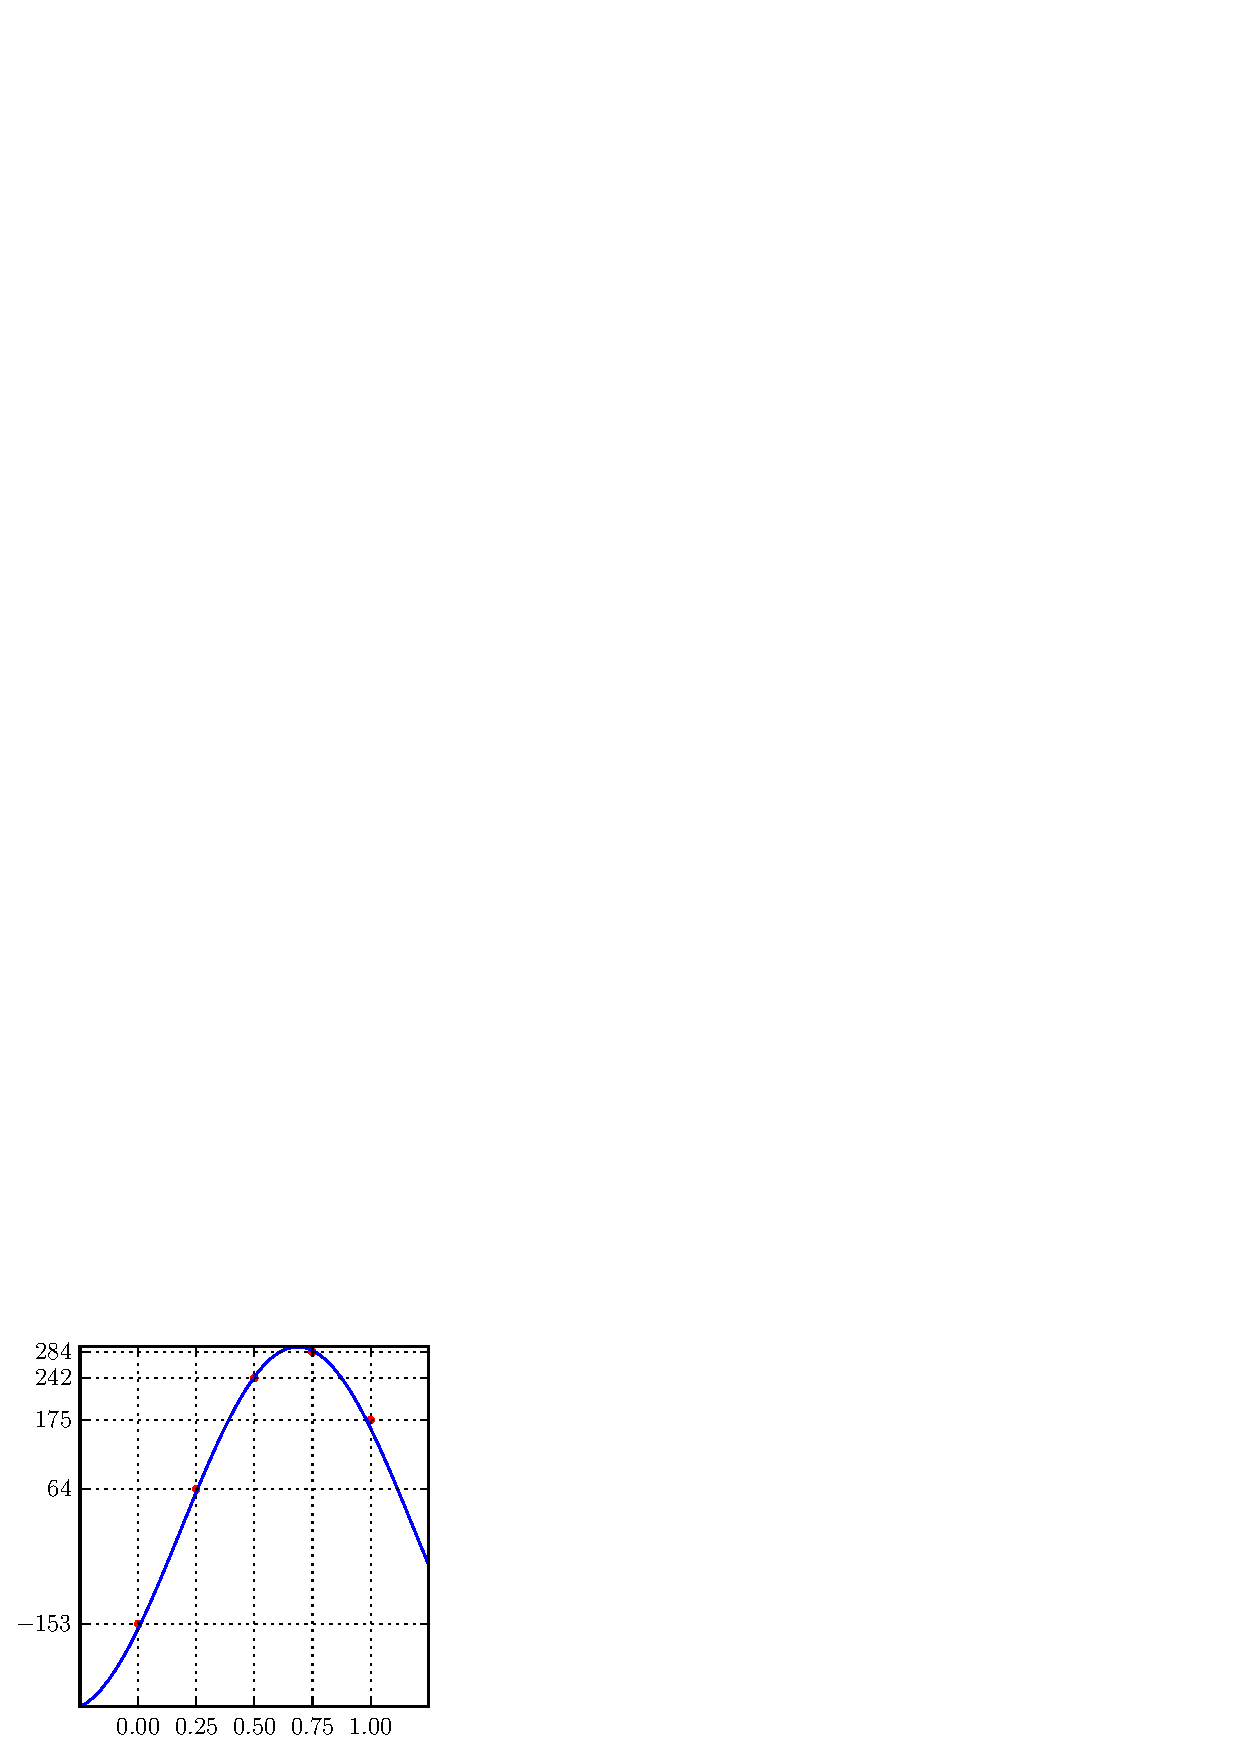
\includegraphics{cap_ajuste/pics/ex_ajuste_linear/ex_ajuste_linear}
  \caption{Gráfico da solução do problema apresentado no exemplo~\ref{ex:ajuste_linear}.}
  \label{fig:ex_ajuste_linear}
\end{figure}


\begin{ex}\label{ex:ajuste_linear} Encontre a função $f(x)=a_1\sen(\pi x) + a_2\cos(\pi x)$ que melhor se ajusta pelo critérios dos mínimos quadrados aos seguintes pontos dados
  \begin{center}
    \begin{tabular}{l|ccccc}
      $i$ & $1$  & $2$ & $3$ & $4$ & $5$\\\hline
      $x_i$ & $0,00$ & $0,25$ & $0,50$ & $0,75$ & $1,00$\\
      $y_i$ & $-153$ & $64$ & $242$ & $284$ & $175$
    \end{tabular}
  \end{center} 
\end{ex}
\begin{sol}
Pelo procedimento visto nesta seção, temos que os coeficientes $a_1$ e $a_2$ são dados pela solução por mínimos quadrados do seguinte sistema linear $Va = y$
\begin{equation*}
  \begin{split}
    a_1\sen(\pi x_1) + a_2\cos(\pi x_1) &= y_1\\
    a_1\sen(\pi x_2) + a_2\cos(\pi x_2) &= y_2\\
    a_1\sen(\pi x_3) + a_2\cos(\pi x_3) &= y_3\\
    a_1\sen(\pi x_4) + a_2\cos(\pi x_4) &= y_4\\
    a_1\sen(\pi x_5) + a_2\cos(\pi x_5) &= y_5
  \end{split}
\end{equation*}
cuja matriz de coeficientes $V$ é:
\begin{equation*}
  V=\begin{bmatrix}
    \sin(0) & \cos(0)  \\
    \sin(0,25\pi) & \cos(0,25\pi)  \\
    \sin(0,5\pi) & \cos(0,5\pi)  \\
    \sin(0,75\pi) & \cos(0,75\pi)  \\
    \sin(\pi) & \cos(\pi)  \\
 \end{bmatrix}
\end{equation*}

Então, a solução por mínimos quadrados é
\begin{equation*}
  a = (V^TV)^{-1}V^Ty =
  \begin{bmatrix}
    244,03658\\
    -161,18783
  \end{bmatrix}.
\end{equation*}
Ou seja, $f(x) = 244,03658\sen(\pi x) - 161,18783\cos(\pi x)$ é a função ajustada ao conjunto de pontos dados. A figura~\ref{fig:ex_ajuste_linear} apresenta o gráfica de $f(x)$ e dos pontos dados.

%%%%%%%%%%%%%%%%%%%%
% scilab
%%%%%%%%%%%%%%%%%%%%
\ifisscilab
No \verb+Scilab+, podemos computar os coeficientes da função $f(x)$ da seguinte forma:
\begin{verbatim}
-->xi = [0 0.25 0.5 0.75 1]';  
-->yi = [-153 64 242 284 175]'; 
-->V = [sin(%pi*xi) cos(%pi*xi)]; 
-->a = inv(V'*V)*V'*yi 
 a  =
    244.03658  
  - 161.18783  
\end{verbatim}
\fi
%%%%%%%%%%%%%%%%%%%%
%%%%%%%%%%%%%%%%%%%%
% octave
%%%%%%%%%%%%%%%%%%%%
\ifisoctave
No \verb+GNU Octave+, podemos computar os coeficientes da função $f(x)$ da seguinte forma:
\begin{verbatim}
xi = [0 0.25 0.5 0.75 1]';
yi = [-153 64 242 284 175]';
V = [sin(pi*xi) cos(pi*xi)];
a = inv(V'*V)*V'*yi
\end{verbatim}
o que nos fornece no {\it prompt}:
\begin{verbatim}
a =
   244.04
  -161.19
\end{verbatim}
\fi
%%%%%%%%%%%%%%%%%%%%
%%%%%%%%%%%%%%%%%%%%
% python
%%%%%%%%%%%%%%%%%%%%
\ifispython
Em \verb+Python+, podemos computar os coeficientes da função $f(x)$ da seguinte forma:
\begin{verbatim}
>>> xi = np.array([0,0.25,0.5,0.75,1])
>>> yi = np.array([-153,64,242,284,175])
>>> V = np.array([np.sin(np.pi*xi),np.cos(np.pi*xi)]).transpose()
>>> a = ((np.linalg.inv((V.transpose()).dot(V))).dot(V.transpose())).dot(yi)
\end{verbatim}
\fi
%%%%%%%%%%%%%%%%%%%%

% A tabela abaixo mostra os valores dados e os valores ajustados:
% \begin{center}
% \begin{tabular}{|c|c|c|c|}
% \hline
% $x_i$ & $y_i$& $f(x_i)$& $f(x_i)-y_i$\\
% \hline
% 0  &   -153&  - 161,18783&  -8,1878306 \\ 
% 0,25&    64 &    58,582912&  -5,4170876 \\ 
% 0,5 &    242&    244,03658&   2,0365799 \\ 
% 0,75&    284&    286,53693&   2,5369286 \\ 
% 1   &    175&    161,18783&  -13,812169 \\
% \hline
% \end{tabular}  
% \end{center}
\end{sol}

%%%%%%%%%%%%%%%%%%%%
% scilab
%%%%%%%%%%%%%%%%%%%%
\ifisscilab
\begin{obs}
  No \verb+Scilab+, quando resolvemos um sistema $Ax = b$ usando
\begin{verbatim}
-->x = inv(A)*b
\end{verbatim}
estamos computando a inversa da matriz $A$ e multiplicando por $b$. Podemos evitar a computação da inversa de $A$ usando o operador contra-barra ($/$). Neste caso, escrevemos
\begin{verbatim}
-->x = A/b
\end{verbatim}
Quando o sistema $A$ não é uma matriz quadrada, \verb+A/b+ retorna a solução por mínimos quadrados do sistema $Ax = b$, enquanto \verb+inv(A)*b+ retorna um erro, pois $A$ não é uma matriz quadrada e, portanto, não é invertível.
\end{obs}
\fi
%%%%%%%%%%%%%%%%%%%%
%%%%%%%%%%%%%%%%%%%%
% octave
%%%%%%%%%%%%%%%%%%%%
\ifisoctave
\begin{obs}
  No \verb+GNU octave+, quando resolvemos um sistema $Ax = b$ usando
\begin{verbatim}
>> x = inv(A)*b
\end{verbatim}
estamos computando a inversa da matriz $A$ e multiplicando por $b$. Podemos evitar a computação da inversa de $A$ usando o operador contra-barra ($/$). Neste caso, escrevemos
\begin{verbatim}
>> x = A/b
\end{verbatim}
Quando o sistema $A$ não é uma matriz quadrada, \verb+A/b+ retorna a solução por mínimos quadrados do sistema $Ax = b$, enquanto \verb+inv(A)*b+ retorna um erro, pois $A$ não é uma matriz quadrada e, portanto, não é invertível.
\end{obs}
\fi
%%%%%%%%%%%%%%%%%%%%
%%%%%%%%%%%%%%%%%%%%
% python
%%%%%%%%%%%%%%%%%%%%
\ifispython
\begin{obs}
  Em \verb+Python+, quando resolvemos um sistema $Ax = b$ usando
\begin{verbatim}
>>> x = np.linalg.inv(A).dot(b)
\end{verbatim}
estamos computando a inversa da matriz $A$ e multiplicando por $b$. Dde forma mais eficiente, podemos usar a função \href{https://docs.scipy.org/doc/numpy/reference/generated/numpy.linalg.solve.html}{numpy.linalg.solve}, digitando:
\begin{verbatim}
>>> x = np.linalg.solve(A,b)
\end{verbatim}
Isto requer que a matriz $A$ seja quadrada e de posto completo. Alternativamente, para obtermos a solução por mínimos quadrados, podemos usar a função \href{https://docs.scipy.org/doc/numpy/reference/generated/numpy.linalg.lstsq.html}{numpy.linalg.lstsq}. Neste caso, digitamos:
\begin{verbatim}
>>> np.linalg.lstsq(A,b)
\end{verbatim}
\end{obs}
\fi
%%%%%%%%%%%%%%%%%%%%

%Observe que é equivalente ao problema matricial
%\begin{equation}
%   Ma := V^TV a = V^Ty
%\end{equation}


% Considere o sistema linear dado por
% $Ax=b$
% onde $A$ é uma matriz $n\times m$ e $b$ é um vetor de $n$ linhas. Assumimos as seguintes hipóteses:
% \begin{itemize}
% \item $n\geq m$. O número de linhas é igual ou superior ao número de colunas. (Mais equações que incógnitas)
% \item O posto de $A$ é $m$, isto é, existem $m$ linhas L.I. Isso implica que $Av=0$ apenas quando $v=0$
% \end{itemize}

% Neste caso, não seremos necessariamente capazes de encontrar um vetor $x$ que satisfaça exatamente a equação $Ax=b$, pelo que estamos interessamos no problema de encontrar o vetor $x$ (ordem m) que minimiza o erro quadrático dado por:
% \begin{equation}\label{defEm}
% E:=\sum_{j=1}^N \left[z_i- b_i\right]^2
% \end{equation}
% onde $z=Ax$ e $z_i$ é linha $i$ do vetor $z$, dado por:
% \begin{equation}\label{Axi}
% z_j=(Ax)_j=\sum_{j=1}^m a_{ij} x_j,\quad j=1,\cdots,n
% \end{equation}
% onde $a_{ij}$ é o elemento de $A$ na linha $i$ e coluna $j$.
% Substituindo (\ref{Axi}) em (\ref{defEm})
% \begin{equation}\label{erro}
% E:=\sum_{j=1}^N \left[\sum_{j=1}^m a_{ij} x_j- b_i\right]^2
% \end{equation}
% Esta é uma função diferenciável nos coeficientes $x_j$ e portanto todo ponto de mínimo acontece quando $\nabla E=0$, ou seja, quando $$\frac{\partial}{\partial x_l}E=0,\forall 1\leq l \leq m $$

% O que implica a seguinte condição
% \begin{eqnarray*}
% 0=\frac{\partial}{\partial x_l}E=\sum_{j=1}^N 2\left[\sum_{j=1}^m a_{ij} x_j- b_i\right] a_{il}, ~~~l=1,\cdots, m
% \end{eqnarray*}
% Equivalente a
% \begin{eqnarray*}
% \sum_{j=1}^N\sum_{j=1}^m  a_{il}x_j a_{ij}=\sum_{j=1}^Na_{il}b_i,~~~l=1,\cdots, m
% \end{eqnarray*}
% que pode ser reescrito na forma vetorial como:
% \begin{eqnarray}\label{cond_vet}
% \left[
% \begin{array}{c}
% \sum_{j=1}^N\sum_{j=1}^m   a_{i1}x_ja_{ij}\\
% \sum_{j=1}^N\sum_{j=1}^m   a_{i2}x_ja_{ij}\\
% \vdots\\
% \sum_{j=1}^N\sum_{j=1}^m   a_{im}x_ja_{ij}\\
% \end{array}
% \right]
% =
% \left[
% \begin{array}{c}
% \sum_{j=1}^Na_{i1}b_i\\
% \sum_{j=1}^Na_{i2}b_i\\
% \vdots\\
% \sum_{j=1}^Na_{im}b_i
% \end{array}
% \right]
% \end{eqnarray}
% Observamos agora que a expressão (\ref{cond_vet}) é equivalente ao seguinte problema matricial:
% 
% \begin{equation}\framebox[100 pt][c]{$A^TA x = A^Tb$}\end{equation}

\subsection{Ajuste polinomial}\index{ajuste!polimomial}

O \emph{ajuste polinomial} é o caso particular do ajuste linear para \emph{funções polinomiais}, isto é, funções do tipo 
\begin{equation*}
  p(x)=a_1 + a_2 x + \cdots + a_{m}x^{m-1}.
\end{equation*}

Neste caso, a matriz $V$ associada ao ajuste dos pontos $\{(x_1, y_1)$, $(x_2, y_2)$, $(x_3, y_3)$, $\ldots$, $(x_n,y_n)\}$ é dada por:
\begin{equation*}
  V=
\begin{bmatrix}
  1     &    x_1   &   x_1^2& \cdots & x_1^{m-1}\\
  1     &    x_2   &   x_2^2& \cdots & x_2^{m-1}\\
  1     &    x_3   &   x_3^2& \cdots & x_3^{m-1}\\
  \vdots&    \vdots&  & \ddots & \vdots    \\
  1     &    x_n   &   x_n^2& \cdots & x_n^{m-1}
\end{bmatrix}
\end{equation*}
Então, os coeficientes $a_i$, $i = 1, 2, \ldots, m$, são dados pela solução do sistema linear $V^TV a = v^Ty$:
\begin{equation*}
  \underbrace{\begin{bmatrix}
     n     &  \sum\limits_{j=1}^n  x_j   & \cdots & \sum\limits_{j=1}^n x_j^{m-1}\\
     \sum\limits_{j=1}^n x_j   &  \sum\limits_{j=1}^n  x_j^2 &        & \sum\limits_{j=1}^n x_j^{m}\\
     \vdots     &              & \ddots & \vdots    \\
     \sum\limits_{j=1}^n x_j^{m-1} &  \sum\limits_{j=1}^n  x_j^{m} & \cdots & \sum\limits_{j=1}^n x_j^{2m-1}
  \end{bmatrix}}_{V^TV}
  \underbrace{\begin{bmatrix}
     a_1 \\
     a_2 \\
     \vdots \\
     a_{p+1}
  \end{bmatrix}}_{a}=
  \underbrace{\begin{bmatrix}
     \sum\limits_{j=1}^n y_j \\
     \sum\limits_{j=1}^n x_j y_j \\
     \vdots \\
     \sum\limits_{j=1}^n x_j^{m-1} y_j 
  \end{bmatrix}}_{V^Ty}
\end{equation*}

\begin{figure}
  \centering
  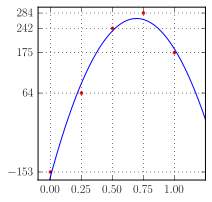
\includegraphics{cap_ajuste/pics/ex_ajuste_polinomial/ex_ajuste_polinomial}
  \caption{Gráfico da solução do problema apresentado no exemplo~\ref{ex:ajuste_polinomial}.}
  \label{fig:ex_ajuste_polinomial}
\end{figure}


\begin{ex}\label{ex:ajuste_polinomial} Entre o polinômio de grau 2 que melhor se ajusta aos pontos dados na seguinte tabela:
  \begin{center}
    \begin{tabular}{l|ccccc}
      $i$ & $1$ & $2$ & $3$ & $4$ & $5$\\\hline
      $x_i$ & $0,00$ & $0,25$ & $0,50$ & $0,75$ & $1,00$\\
      $y_i$ & $-153$ & $64$ & $242$ & $284$ & $175$
    \end{tabular}
  \end{center} 
\end{ex}
\begin{sol}
Um polinômio de grau 2 pode ser escrito na seguinte forma:
\begin{equation*}
  p(x) = a_1 + a_2x + a_3x^2.
\end{equation*}
Assim, o problema se resume em encontrarmos a solução por mínimos quadrados do seguinte sistema linear:
\begin{equation*}
  \begin{split}
  a_1 + a_2x_1 + a_3x_1^2 &= y_1\\
  a_2 + a_2x_2 + a_3x_2^2 &= y_2\\
  a_3 + a_2x_3 + a_3x_3^2 &= y_3\\
  a_4 + a_2x_4 + a_3x_4^2 &= y_4\\
  a_5 + a_2x_5 + a_3x_5^2 &= y_5    
  \end{split}
\end{equation*}
Ou, escrita na forma matricial, $Va = y$, onde:
\begin{equation*}
  V =
  \begin{bmatrix}
    1 & x_1 & x_1^2\\
    1 & x_2 & x_2^2\\
    1 & x_3 & x_3^2\\
    1 & x_4 & x_4^2\\
    1 & x_5 & x_5^2
  \end{bmatrix}
\end{equation*}

A solução por mínimos quadrados é, então:
\begin{equation*}
  a = (V^TV)^{-1}V^Ty =
  \begin{bmatrix}
    - 165,37143 \\
    1250,9714  \\
  - 900,57143  
  \end{bmatrix}
\end{equation*}
Ou seja, o polinômio de grau 2 que melhor ajusta os pontos dados no sentido de mínimos quadrados é $p(x) = -165,37143 + 1250,9714x -900,57143x^2$. A figura~\ref{fig:ex_ajuste_polinomial} mostra o gráfico do polinômio ajustado e os pontos dados.

%%%%%%%%%%%%%%%%%%%%
% scilab
%%%%%%%%%%%%%%%%%%%%
\ifisscilab
No \verb+Scilab+, podemos computar o polinômio $p(x)$ da seguinte forma:
\begin{verbatim}
-->xi = [0 0.25 0.5 0.75 1]';
-->yi = [-153 64 242 284 175]';
-->V = [ones(5,1) xi xi.^2];
-->a = V\yi;
-->p = poly(a,'x','c') 
 p  =
                                       2  
  - 165.37143 + 1250.9714x - 900.57143x   
\end{verbatim}
Para fazermos o gráfico do polinômio e dos pontos, digitamos:
\begin{verbatim}
-->xx = linspace(-0.25,1.25); 
-->plot(xi,yi,'ro',xx,horner(p,xx),'b-');xgrid
\end{verbatim}
\fi
%%%%%%%%%%%%%%%%%%%%
%%%%%%%%%%%%%%%%%%%%
% octave
%%%%%%%%%%%%%%%%%%%%
\ifisoctave
No \verb+GNU Octave+, podemos computar o polinômio $p(x)$ da seguinte forma:
\begin{verbatim}
>> xi = [0 0.25 0.5 0.75 1]';
>> yi = [-153 64 242 284 175]';
>> V = [xi.^2 xi xi.^0];
>> a = V\yi
a =

   -900.57
   1250.97
   -165.37
\end{verbatim}
Para fazermos o gráfico do polinômio e dos pontos, digitamos:
\begin{verbatim}
>> xx = linspace(-0.25,1.25);
>> plot(xi,yi,'ro',xx,polyval(a,xx),'b-');grid on
\end{verbatim}
\fi
%%%%%%%%%%%%%%%%%%%%
%%%%%%%%%%%%%%%%%%%%
% python
%%%%%%%%%%%%%%%%%%%%
\ifispython
Em \verb+Python+, podemos computar os coeficientes do polinômio $p(x)$ da seguinte forma:
\begin{verbatim}
>>> xi = np.array([0,0.25,0.5,0.75,1])
>>> yi = np.array([-153,64,242,284,175])
>>> V = np.array([xi**2,xi**1,xi**0]).transpose()
>>> a = ((np.linalg.inv((V.transpose()).dot(V))).dot(V.transpose())).dot(yi)
\end{verbatim}
Para fazermos o gráfico do polinômio e dos pontos, digitamos:
\begin{verbatim}
>>> xx = np.linspace(-0.25,1.25)
>>> plt.plot(xi,yi,'ro',xx,np.polyval(a,xx),'b-')
>>> plt.grid();plt.show()
\end{verbatim}
\fi
%%%%%%%%%%%%%%%%%%%%
\end{sol}

% 
% Dado um conjunto de $n$ pontos, desejamos encontrar o \textit{polinômio} de grau $p$ que melhor se ajusta a esses pontos de tal forma a minimizar o resíduo, ou seja, encontrar a curva $f(x)=a_1+a_2 x+...+a_{p+1}x^{p}$ tal que 
% \begin{eqnarray*}
%   R(a_1,...,a_{p+1}) &=&\sum_{j=1}^N (f(x_j)-y_j)^2 \\
%                  &=&\sum_{j=1}^N (a_1 + a_2 x_j+...+a_{p+1}x_j^p-y_j)^2
% \end{eqnarray*}
% seja o menor possível.
% 
% O objetivo é encontrar as incógnitas $a_i$ que minimizam a soma do quadrado do resíduo.
% 
% O mínimo de $R$ encontra-se quando a derivada primeira é igual a zero:
% \begin{eqnarray*}
%   \frac{\partial R}{\partial a_1}     &=& \frac{\partial }{\partial a_1}     \sum_{j=1}^n (a_1 + a_2 x_j+...+a_{p+1}x_j^p-y_j)^2 =0 \\
%   \vdots &=& \vdots \\
%   \frac{\partial R}{\partial a_{p+1}} &=& \frac{\partial }{\partial a_{p+1}} \sum_{j=1}^n (a_1 + a_2 x_j+...+a_{p+1}x_j^p-y_j)^2 =0 
% \end{eqnarray*}
% ou seja,
% \begin{eqnarray*}
%    2 \sum_{j=1}^n (a_1 + a_2 x_j+...+a_{p+1}x_j^p-y_j)\cdot 1    &=&0 \\
%   \vdots &=& \vdots \\
%    2 \sum_{j=1}^n (a_1 + a_2 x_j+...+a_{p+1}x_j^p-y_j)\cdot x_j^p&=&0 
% \end{eqnarray*}
% e isolando as incógnitas temos
% \begin{eqnarray*}
%    a_1\sum_{j=1}^n 1     + a_2 \sum_{j=1}^Nx_j      +...+a_{p+1} \sum_{j=1}^Nx_j^{p} &=\sum_{j=1}^N y_j\\
%   \vdots &= \vdots \\
%    a_1\sum_{j=1}^n x_j^p + a_2 \sum_{j=1}^Nx_j^{p+1}+...+a_{p+1} \sum_{j=1}^Nx_j^{2p} &=\sum_{j=1}^N y_jx_j^{p}
% \end{eqnarray*}
% 
% Na forma matricial obtemos
% \begin{equation}
%   \begin{bmatrix}
%      \sum 1     &  \sum  x_j   & \cdots & \sum x_j^p\\
%      \sum x_j   &  \sum  x_j^2 &        & \sum x_j^{p+1}\\
%      \vdots     &              & \ddots & \vdots    \\
%      \sum x_j^p &  \sum  x_j^{p+1} & \cdots & \sum x_j^{2p}
%   \end{bmatrix}
%   \begin{bmatrix}
%      a_1 \\
%      a_2 \\
%      \vdots \\
%      a_{p+1}
%   \end{bmatrix}=
%   \begin{bmatrix}
%      \sum y_j \\
%      \sum x_j y_j \\
%      \vdots \\
%      \sum x_j^p y_j 
%   \end{bmatrix}
% \end{equation}
% 
% Na forma matricial temos 
% \begin{equation}
%    Ma := V^TV a = V^Ty
% \end{equation}
% 

\subsection*{Exercícios}

\begin{exer}
  Encontre o polinômio $p(x) = a_1 + a_2x + a_3x^2$ que melhor se ajusta no sentido de mínimos quadrados aos pontos:
  \begin{center}
    \begin{tabular}{l|cccc}
      $i$ & $1$ & $2$ & $3$ & $4$ \\\hline
      $x_i$ & $-1,50$ & $-0,50$ & $1,25$ & $1,50$\\
      $y_i$ & $1,15$ & $-0,37$ & $0,17$ & $0,94$
  \end{tabular} 
    \end{center}
\end{exer}
\begin{resp}
    $a_1 = -0,1946029$, $a_2 = 0,585986$, $a_3 = -0,0112599$. 
\end{resp}

\begin{exer}Encontrar a parábola $y=ax^2+bx+c$ que melhor aproxima o seguinte conjunto de dados:
  \begin{center}
    \begin{tabular}{l|ccccc}
      $i$ & $1$ & $2$ & $3$ & $4$ & $5$ \\\hline
      $x_i$ & $0,01$ & $1,02$ & $2,04$ & $2,95$ & $3,55$\\
      $y_i$ & $1,99$ & $4,55$ & $7,20$ & $9,51$ & $10,82$
    \end{tabular}
  \end{center} 
\end{exer}
\begin{resp}  
    $y=-0,0407898x^2+ 2,6613293x+ 1,9364598$.
\end{resp}

\begin{exer} Dado o seguinte conjunto de dados
  \begin{center}
    \begin{tabular}{l|ccccccccccc}
      $x_i$ & $0,0$ & $0,1$ & $0,2$ & $0,3$ & $0,4$ & $0,5$ & $0,6$ & $0,7$ & $0,8$ & $0,9$ & $1,0$\\\hline
      $y_i$ & $31$ & $35$ & $37$ & $33$ & $28$ & $20$ & $16$ & $15$ & $18$ & $23$ & $31$
    \end{tabular}
  \end{center} 
\begin{enumerate}[a)]
\item Encontre a função do tipo $f(x)=a+b\sin(2\pi x)+c\cos(2\pi x)$ que melhor aproxima os valores dados.
\item Encontre a função do tipo $f(x)=a+bx+cx^2+dx^3$ que melhor aproxima os valores dados.
\end{enumerate}
\end{exer}
\begin{resp}
    a) $a=25,638625$, $b=9,8591874$, $c=4,9751219$; b)$a=31,475524$, $b=65,691531$, $c=-272,84382$, $d=208,23621$.
\end{resp}



% \begin{exer}Encontre a partir de primeiros princípios a função do tipo $f(x)=bx+a$ que melhor aproxima os pontos:
%   \begin{equation*}
%     (0,-0,1), (1,~2), (2,~3,7) ~ \text{e} ~(3,~7).  
%   \end{equation*}
% \end{exer}
% \begin{resp}
% \begin{eqnarray*}
% E_q&=&[f(0)+0,1]^2+[f(1)-2]^2+[f(2)-3,7]^2+[f(3)-7]^2\\
% &=&[a+0,1]^2+[a+b-2]^2+[a+2b-3,7]^2+[a+3b-7]^2
% \end{eqnarray*}

% Devemos encontrar os parâmetros $a$ $b$ que minimizam o erro, por isso, calculamos as derivadas parciais:
% \begin{eqnarray*}
% \frac{\partial E_q}{\partial a}&=&2[a+0,1]+2[a+b-2]+2[a+2b-3,7]+2[a+3b-7]\\
% \frac{\partial E_q}{\partial b}&=&2[a+b-2]+4[a+2b-3,7]+6[a+3b-7]
% \end{eqnarray*}



% O erro mínimo acontece quando as derivadas são nulas, ou seja:
% \begin{eqnarray*}
% 8a+12b&=&25,2\\
% 12a+28b&=&60,8
% \end{eqnarray*}
% Cuja solução é dada por $a=-0,3$ e $b=2,3$.
% Portanto a função que procuramos é $f(x)=-0,3 +2,3x$.  
% \end{resp}



% \begin{exer} Encontre a função do tipo $f(x)=ax$ que melhor se aproxima dos seguintes pontos:
%   \begin{equation*}
%     (0, -0,1), (1, 2), (2, 3,7) ~ \text{e} ~(3, 7).  
%   \end{equation*}
% \end{exer}
% \begin{resp}
% Defina $$E_q=[f(x_1)-y_1]^2+[f(x_2)-y_2]^2+[f(x_3)-y_3]^2+[f(x_4)-y_4]^2$$
% temos que
% \begin{eqnarray*}
% E_q&=&[f(0)+0,1]^2+[f(1)-2]^2+[f(2)-3,7]^2+[f(3)-7]^2\\
% &=&[0,1]^2+[a-2]^2+[2a-3,7]^2+[3a-7]^2
% \end{eqnarray*}

% Devemos encontrar o parâmetro $a$ que minimiza o erro, portanto, calculamos:
% \begin{eqnarray*}
% \frac{\partial E_q}{\partial a}&=&2[a-2]+4[2a-3,7]+6[3a-7]=28a-60,8
% \end{eqnarray*}
% Portanto o valor de $a$ que minimiza o erro é $a=\frac{60,8}{28}$.
% \ifisscilab
% \begin{verbatim}
% x=[0 1 2 3]'
% y=[-.1 2 3.7 7]'
% plot2d(x,y,style=-4)
% \end{verbatim}
% \fi
% \end{resp}


\section{Aproximando problemas não lineares por problemas lineares}

Eventualmente, problemas de ajuste de curvas podem recair em um sistema não linear. Por exemplo, para ajustar função $y=Ae^{bx}$ ao conjunto de pontos $(x_1,y_1)$, $(x_2,y_2)$ e $(x_3,y_3)$, temos que minimizar o resíduo\footnote{A soma do quadrado dos resíduos.} 
$$
R=(Ae^{x_1b}-y_1)^2+(Ae^{x_2b}-y_2)^2+(Ae^{x_3b}-y_3)^2
$$
ou seja, resolver o sistema
\begin{eqnarray*}
\frac{\partial R}{\partial A} &=& 2(Ae^{x_1b}-y_1)e^{x_1b}+2(Ae^{x_2b}-y_2)e^{x_2b}+2(Ae^{x_3b}-y_3)e^{x_3b}=0\\
\frac{\partial R}{\partial b} &=& 2Ax_1(Ae^{x_1b}-y_1)e^{x_1b} + 2Ax_2(Ae^{x_2b}-y_2)e^{x_2b} \\
&+& 2Ax_3(Ae^{x_3b}-y_3)e^{x_3b}=0
\end{eqnarray*}
que é não linear em $A$ e $b$. Esse sistema pode ser resolvido pelo método de Newton-Raphson, o que pode se tornar custoso, ou mesmo inviável quando não dispomos de uma boa aproximação da solução para inicializar o método.

Felizmente, algumas famílias de curvas admitem uma transformação que nos leva a um problema linear. No caso da curva $y=Ae^{bx}$, observe que $\ln y=\ln A+bx$. Assim, em vez de ajustar a curva original $y=Ae^{bx}$ a tabela de pontos, ajustamos a curva submetida a transformação logarítmica
$$
\tilde y:=a_1+a_2 \tilde x=\ln A+bx.
$$
Usamos os pontos $(\tilde x_j,\tilde y_j):=(x_j,\ln y_j)$, $j=1,2,3$ e resolvemos o sistema linear
$$
V^T V \left[\begin{array}{c} a_1\\a_2 \end{array}\right]=V^T\left[\begin{array}{c}\tilde{y}_1\\\tilde{y}_2\\\tilde{y}_3 \end{array}\right],
$$
onde
$$
A=\left[\begin{array}{cc} 1&x_1\\1&x_2\\1&x_3 \end{array}\right]
$$
\begin{ex}Encontre uma curva da forma $y=Ae^x$ que melhor ajusta os pontos $(1, 2)$, $(2, 3)$ e $(3, 5)$.
\end{ex}
Temos
$$
A=\left[\begin{array}{cc} 1&1\\1&2\\1&3 \end{array}\right]
$$
e a solução do sistema leva em $B=0,217442$ e $b=0,458145$. Portanto, $A=e^{0,217442}=1,24289$.

\begin{obs}
Os coeficientes obtidos a partir dessa linearização são aproximados, ou seja, são diferentes daqueles obtidos quando aplicamos mínimos quadrados não linear. Observe que estamos minimizando $\displaystyle\sum_i [\ln y_i -\ln (f(x_i))]^2$ em vez de $\displaystyle\sum_i [ y_i -f(x_i)]^2$. No exemplo resolvido, a solução do sistema não linear original seria $A=1,19789$ e $b=0,474348$
\end{obs}

\begin{obs}
Mesmo quando se deseja resolver o sistema não linear, a solução do problema linearizado pode ser usada para construir condições iniciais.
\end{obs}


A próxima tabela apresenta algumas curvas e transformações que linearizam o problema de ajuste.
\begin{center}
  \begin{tabular}{|c|c|c|}\hline
Curva    & Transformação & Problema Linearizado\\ \hline
$\displaystyle y=ae^{bx}$       & $\tilde y=\ln y$   & $\tilde y=\ln a+ bx$\\
$\displaystyle y=ax^b $       &$\tilde y=\ln y$   & $\tilde y=\ln a+ b\ln x$\\
$\displaystyle y=ax^be^{cx}$    &$\tilde y=\ln y$  & $\tilde y=\ln a+ b\ln x+cx$\\
$\displaystyle y=ae^{(b+cx)^2}$ &$\tilde y=\ln y$       & $\tilde y=\ln a+b^2+ bc x+c^2x^2$\\
$\displaystyle y=\frac{a}{b+x}$ &$\displaystyle \tilde y=\frac{1}{y}$ & $\displaystyle \tilde y=\frac{b}{a}+\frac{1}{a}x$\\
$y=A\cos(\omega x+\phi)$   & $-x-$ &  $y=a\cos(\omega x)-b\sin(\omega x)$ \\
$\omega\ \text{conhecido} $&   &  $a=A\cos(\phi),\ b=A\sin(\phi)$ \\ \hline    
  \end{tabular}
\end{center}

\begin{ex}
Encontre a função $f$ da forma $y=f(x)=A\cos(2 \pi x+\phi)$ que ajusta a tabela de pontos
\begin{center}
\begin{tabular}{|c|c|}
\hline
$x_i$ & $y_i$\\
\hline
0,0  &   9,12\\
0,1  &    1,42\\
0,2  &  - 7,76\\
0,3  &  - 11,13\\
0,4  &  - 11,6\\
0,5  &  - 6,44\\
0,6  &    1,41\\
0,7  &    11,01\\
0,8  &    14,73\\
0,9  &    13,22\\
1,0  &    9,93 \\
\hline
\end{tabular}  
\end{center}
\end{ex}
\begin{sol}
Usando o fato que $y=A\cos(2 \pi x+\phi)=a\cos(2 \pi x)-b\sin(2 \pi x)$, onde $a=A\cos(\phi)$ e $b=A\sin(\phi)$, $z=[\begin{array}{cc}a &b\end{array}]^T$ é solução do problema
$$
B^TBz=B^Ty,
$$
onde
$$
B\!=\!\left[\begin{array}{cc}\cos(2 \pi x_0)& -\sin(2 \pi x_0)\\ \cos(2 \pi x_1)& -\sin(2 \pi x_1)\\ \vdots\\ \cos(2 \pi x_{10})& -\sin(2\pi x_{10}) \end{array}\right]\!=\!\left[\begin{array}{cc}  1.     &      0.\\
    0,8090170 & - 0,5877853\\
    0,3090170 & - 0,9510565\\
  - 0,3090170 & - 0,9510565\\
  - 0,8090170 & - 0,5877853\\
  - 1,0000000 &   0,0000000\\
  - 0,8090170 &   0,5877853\\
  - 0,3090170 &   0,9510565\\
    0,3090170 &   0,9510565\\
    0,8090170 &   0,5877853\\
    1,0000000 &   0,0000000   \end{array}\right].
$$
Assim, $a=7,9614704$ e $b=11,405721$ e obtemos o seguinte sistema:
$$
\left\{\begin{array}{c}
A\cos(\phi)=7,9614704\\ A\sin(\phi)=11,405721
\end{array}\right..
$$
Observe que
$$
A^2=7,9614704^2+11,405721^2
$$
e, escolhendo $A>0$, $A=13,909546$ e
$$
\sin(\phi)=\frac{11,405721}{13,909546}=0,8199923
$$
Assim, como $\cos\phi$ também é positivo, $\phi$ é um ângulo do primeiro quadrante:
$$
\phi=0,9613976
$$
Portanto $f(x)=13,909546\cos(2\pi x+0,9613976)$. Observe que nesse exemplo a solução do problema linear é a mesma do problema não linear.  
\end{sol}

\begin{ex}
Encontre a função $f$ da forma $y=f(x)=\frac{a}{b+x}$ que ajusta a tabela de pontos
$$
\begin{tabular}{|c|c|}
\hline
$x_i$ & $y_i$\\
\hline
0,0  & 101\\
0,2  &  85\\
0,4  &  75\\
0,6  &  66\\
0,8  &  60\\
1,0  &  55 \\
\hline
\end{tabular}
$$
usando uma das transformações tabeladas.
\end{ex}
\begin{sol}
Usando o fato que $Y=\frac{1}{y}=\frac{b}{a}+\frac{1}{a}x$, $z=[\begin{array}{cc}\frac{b}{a} &\frac{1}{a}\end{array}]^T$ é solução do problema
$$
A^TAz=A^TY,
$$
onde
$$
A=\left[\begin{array}{cc}1& x_1\\ 1& x_2\\ 1&x_3\\1&x_4 \\ 1&x_5 \\ 1&x_6 \end{array}\right]=\left[\begin{array}{cc}
  1 &  0,0\\
  1 &  0,2\\
  1 &  0,4\\
  1 &  0,6\\
  1 &  0,8\\
  1 &  1,0
\end{array}\right]
$$
e
$$
Y=\left[\begin{array}{c}
  1/y_1\\
    1/y_2\\
    1/y_3\\
    1/y_4\\
    1/y_5\\
    1/y_6
\end{array}\right]=\left[\begin{array}{c}
  0,0099010\\
  0,0117647\\
  0,0133333\\
  0,0151515\\
  0,0166667\\
  0,0181818
\end{array}\right]
$$
Assim, $\frac{1}{a}=0,0082755$ e $\frac{b}{a}=0,0100288$ e, então, $a=120,83924$ e $b=1,2118696$, ou seja, $f(x)=\frac{120,83924}{1,2118696+x}$.  
\end{sol}

%\end{document} 
